\chapter{Development documentation}
\label{chap:development_documentation}

In this chapter first, we present the overall architecture of our software application. Then, for the frontend and the backend we describe the main libraries that we used and we describe our code structure. Finally, we show our LLM assistant server architecture and its work-flow.


\section{Overall architecture}

Figure \ref{fig:complete_overview} shows the architecture of the whole software application that implements the high-level architecture presented in the section \ref{sec:high_level_architecture}. The architecture consists of its own frontend and its own backend. The frontend is additionally integrated with the Dataspecer tool\footnote{\url{https://dataspecer.com/}} for management of the domain models. The backend is divided into the \emph{LLM assistant server} component and the \emph{LLM server} component.

\begin{figure}[!h]
    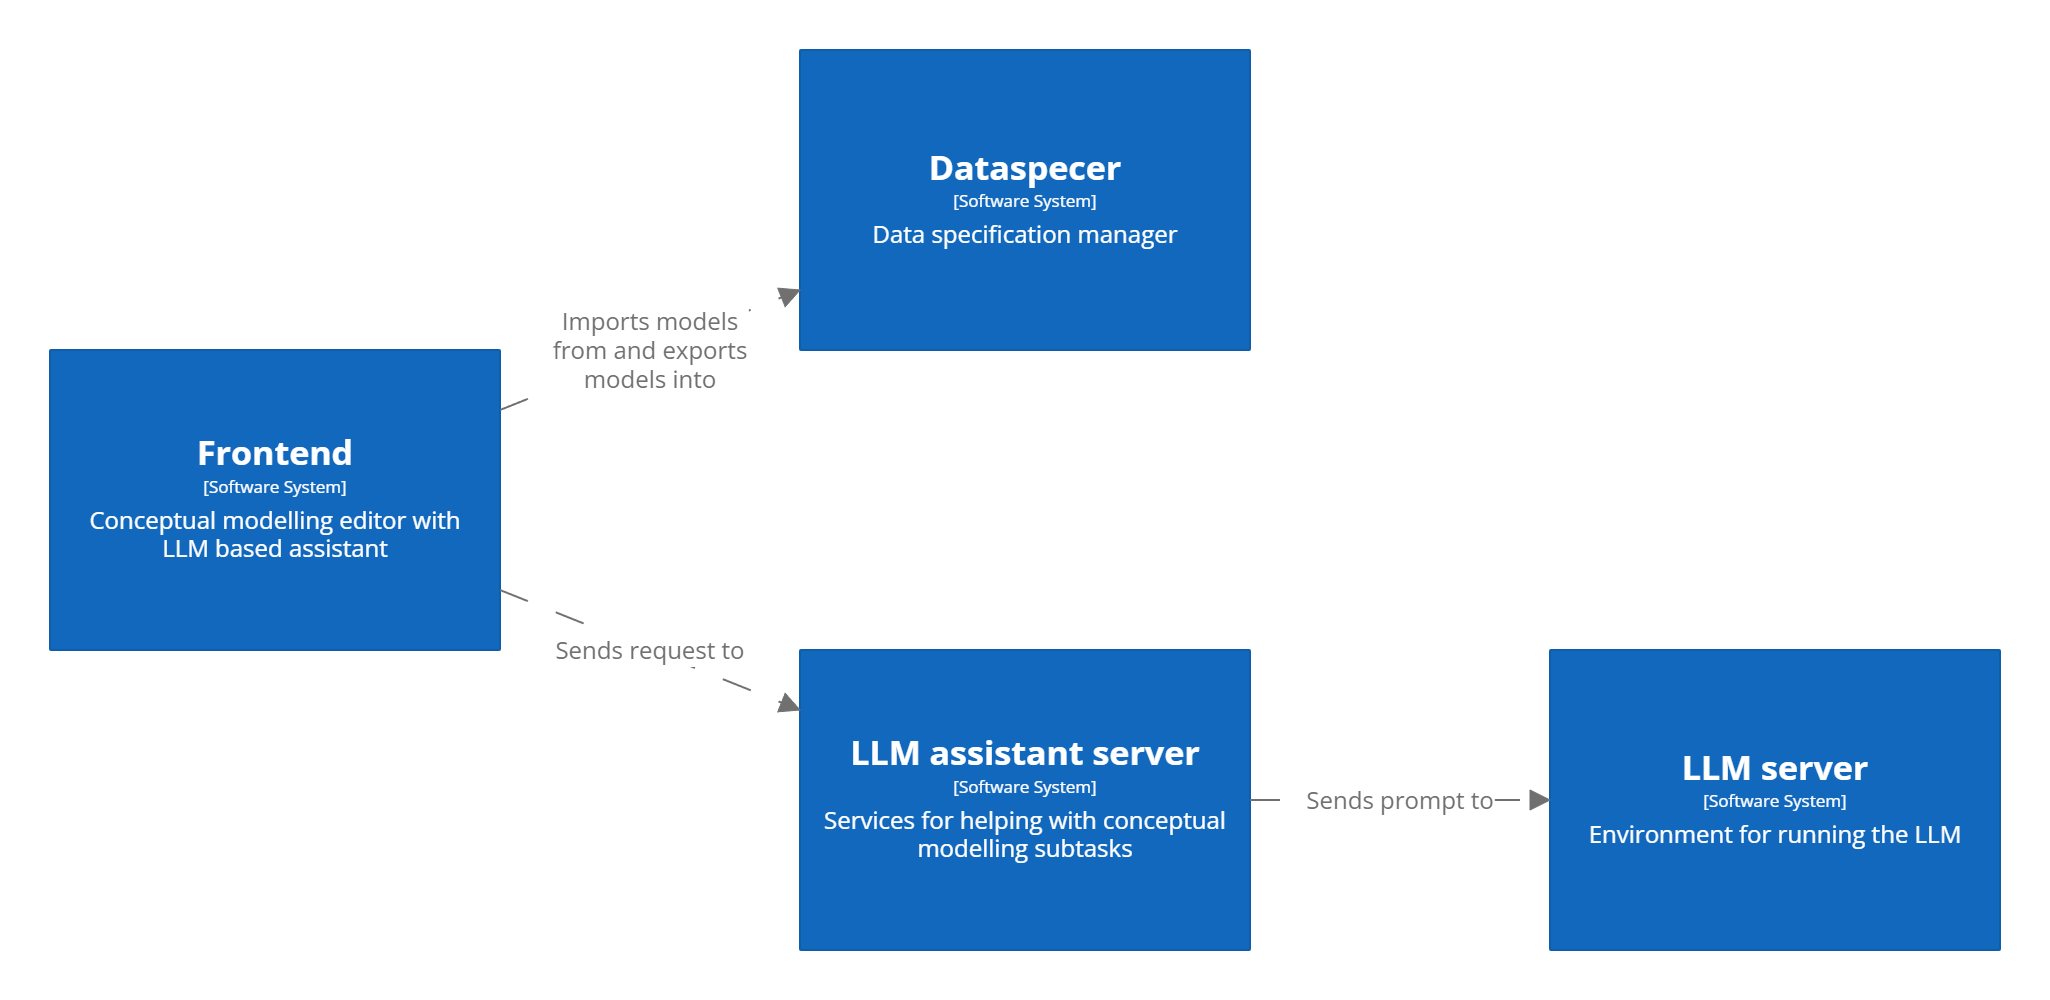
\includegraphics[scale=0.20]{../docs/images/architecture/complete-overview.png}
    \caption{\centering Complete architecture overview}
    \label{fig:complete_overview}
\end{figure}


\section{Frontend}

\noindent{}The frontend is developed with:
\begin{itemize}
\item Node.js\footnote{\url{https://nodejs.org/en}} version 21.5.0
\item React\footnote{\url{https://react.dev/}} version 18.2.0
\item Typescript\footnote{\url{https://www.typescriptlang.org/}} version 4.9.5
\end{itemize}


\subsection{Main libraries}

\noindent{}We used mainly the following libraries:
\begin{itemize}
\item React Flow\footnote{\url{https://reactflow.dev/}} for displaying the domain models
\item Recoil\footnote{\url{https://recoiljs.org/}} for state management
\item Material UI\footnote{\url{https://mui.com/}} for UI design
\end{itemize}


\subsection{Code structure}

\noindent{}The structure of the code is divided into the following directories:
\begin{itemize}
\item \textit{atoms} contain Recoil states
\item \textit{components} contain all the building blocks of the application, the main components are:
\begin{itemize}
\item \textit{ConceptualModel} for working with the domain model
\item \textit{Topbar} and \textit{Sidebar} mainly for displaying to the user the suggestions from the LLM assistant
\end{itemize}
\item \textit{definitions} contain definitions of the constant variables, interfaces, enums, and custom types, the most important scripts are:
\begin{itemize}
\item \textit{fetch.ts}: defines the interfaces for communicating with the LLM assistant server based on the API endpoints documentation\footnote{\url{https://github.com/Dominik7131/Conceptual-Modeling-LLM-Assistant/blob/master/docs/api-endpoints.md}}
\item \textit{urls.ts}: defines the endpoints used for communicating with the LLM assistant server based on the mentioned API endpoints documentation
\end{itemize}
\item \textit{hooks} contain custom hooks mainly for fetching the data from the LLM assistant server
\item \textit{utils} contain functions usually used by more than one component
\end{itemize}


\noindent{}For additional information, see our frontend development documentation\footnote{\url{https://github.com/Dominik7131/Conceptual-Modeling-LLM-Assistant/blob/master/docs/frontend-dev.md}}. For information about frontend installation see our fronted installation documentation\footnote{\url{https://github.com/Dominik7131/Conceptual-Modeling-LLM-Assistant/blob/master/frontend/conceptual-model-editor-assistant/README.md\#how-to-run}}.


\section{Backend}

\noindent{}The LLM assistant server uses:
\begin{itemize}
\item Flask\footnote{\url{https://flask.palletsprojects.com/en/3.0.x/}} version 3.0.1
\item Python\footnote{\url{https://www.python.org/}} version 3.10
\end{itemize}

\noindent{}The \emph{LLM server} uses llama.cpp server\footnote{\url{https://github.com/ggerganov/llama.cpp/tree/master/examples/server}}. The \emph{LLM assistant server} communicates with this server via OpenAI API\footnote{\url{https://github.com/openai/openai-openapi}}.


\subsection{Code structure}

\noindent{}The code is divided into these main directories:
\begin{itemize}
\item \textit{definitions} contain definitions of constant variables and enums
\item \textit{text-filtering} contain the implementation of the semantic and syntactic RAG approach
\item \textit{utils} contain scripts used by the LLM assistant server
\item \textit{tests} contain scripts for testing correctness of the implementation of some components
\item \textit{data-processing} contain scripts for experimenting with different configurations such as different prompts, RAG approaches, LLMs, etc.
\begin{itemize}
\item scripts in the generation directory are used for generating test data
\item scripts in the evaluation directory are used for evaluating the RAG approaches, the generated domain elements, and the generated descriptions
\end{itemize}
\end{itemize}

\noindent{}For additional information and a more detailed description see our backend development documentation\footnote{\url{https://github.com/Dominik7131/Conceptual-Modeling-LLM-Assistant/blob/master/docs/backend-dev.md}}. For backend installation see our backend installation documentation\footnote{\url{https://github.com/Dominik7131/Conceptual-Modeling-LLM-Assistant/blob/master/backend/README.md}}.


\subsection{LLM assistant server architecture}

\begin{figure}[!h]
    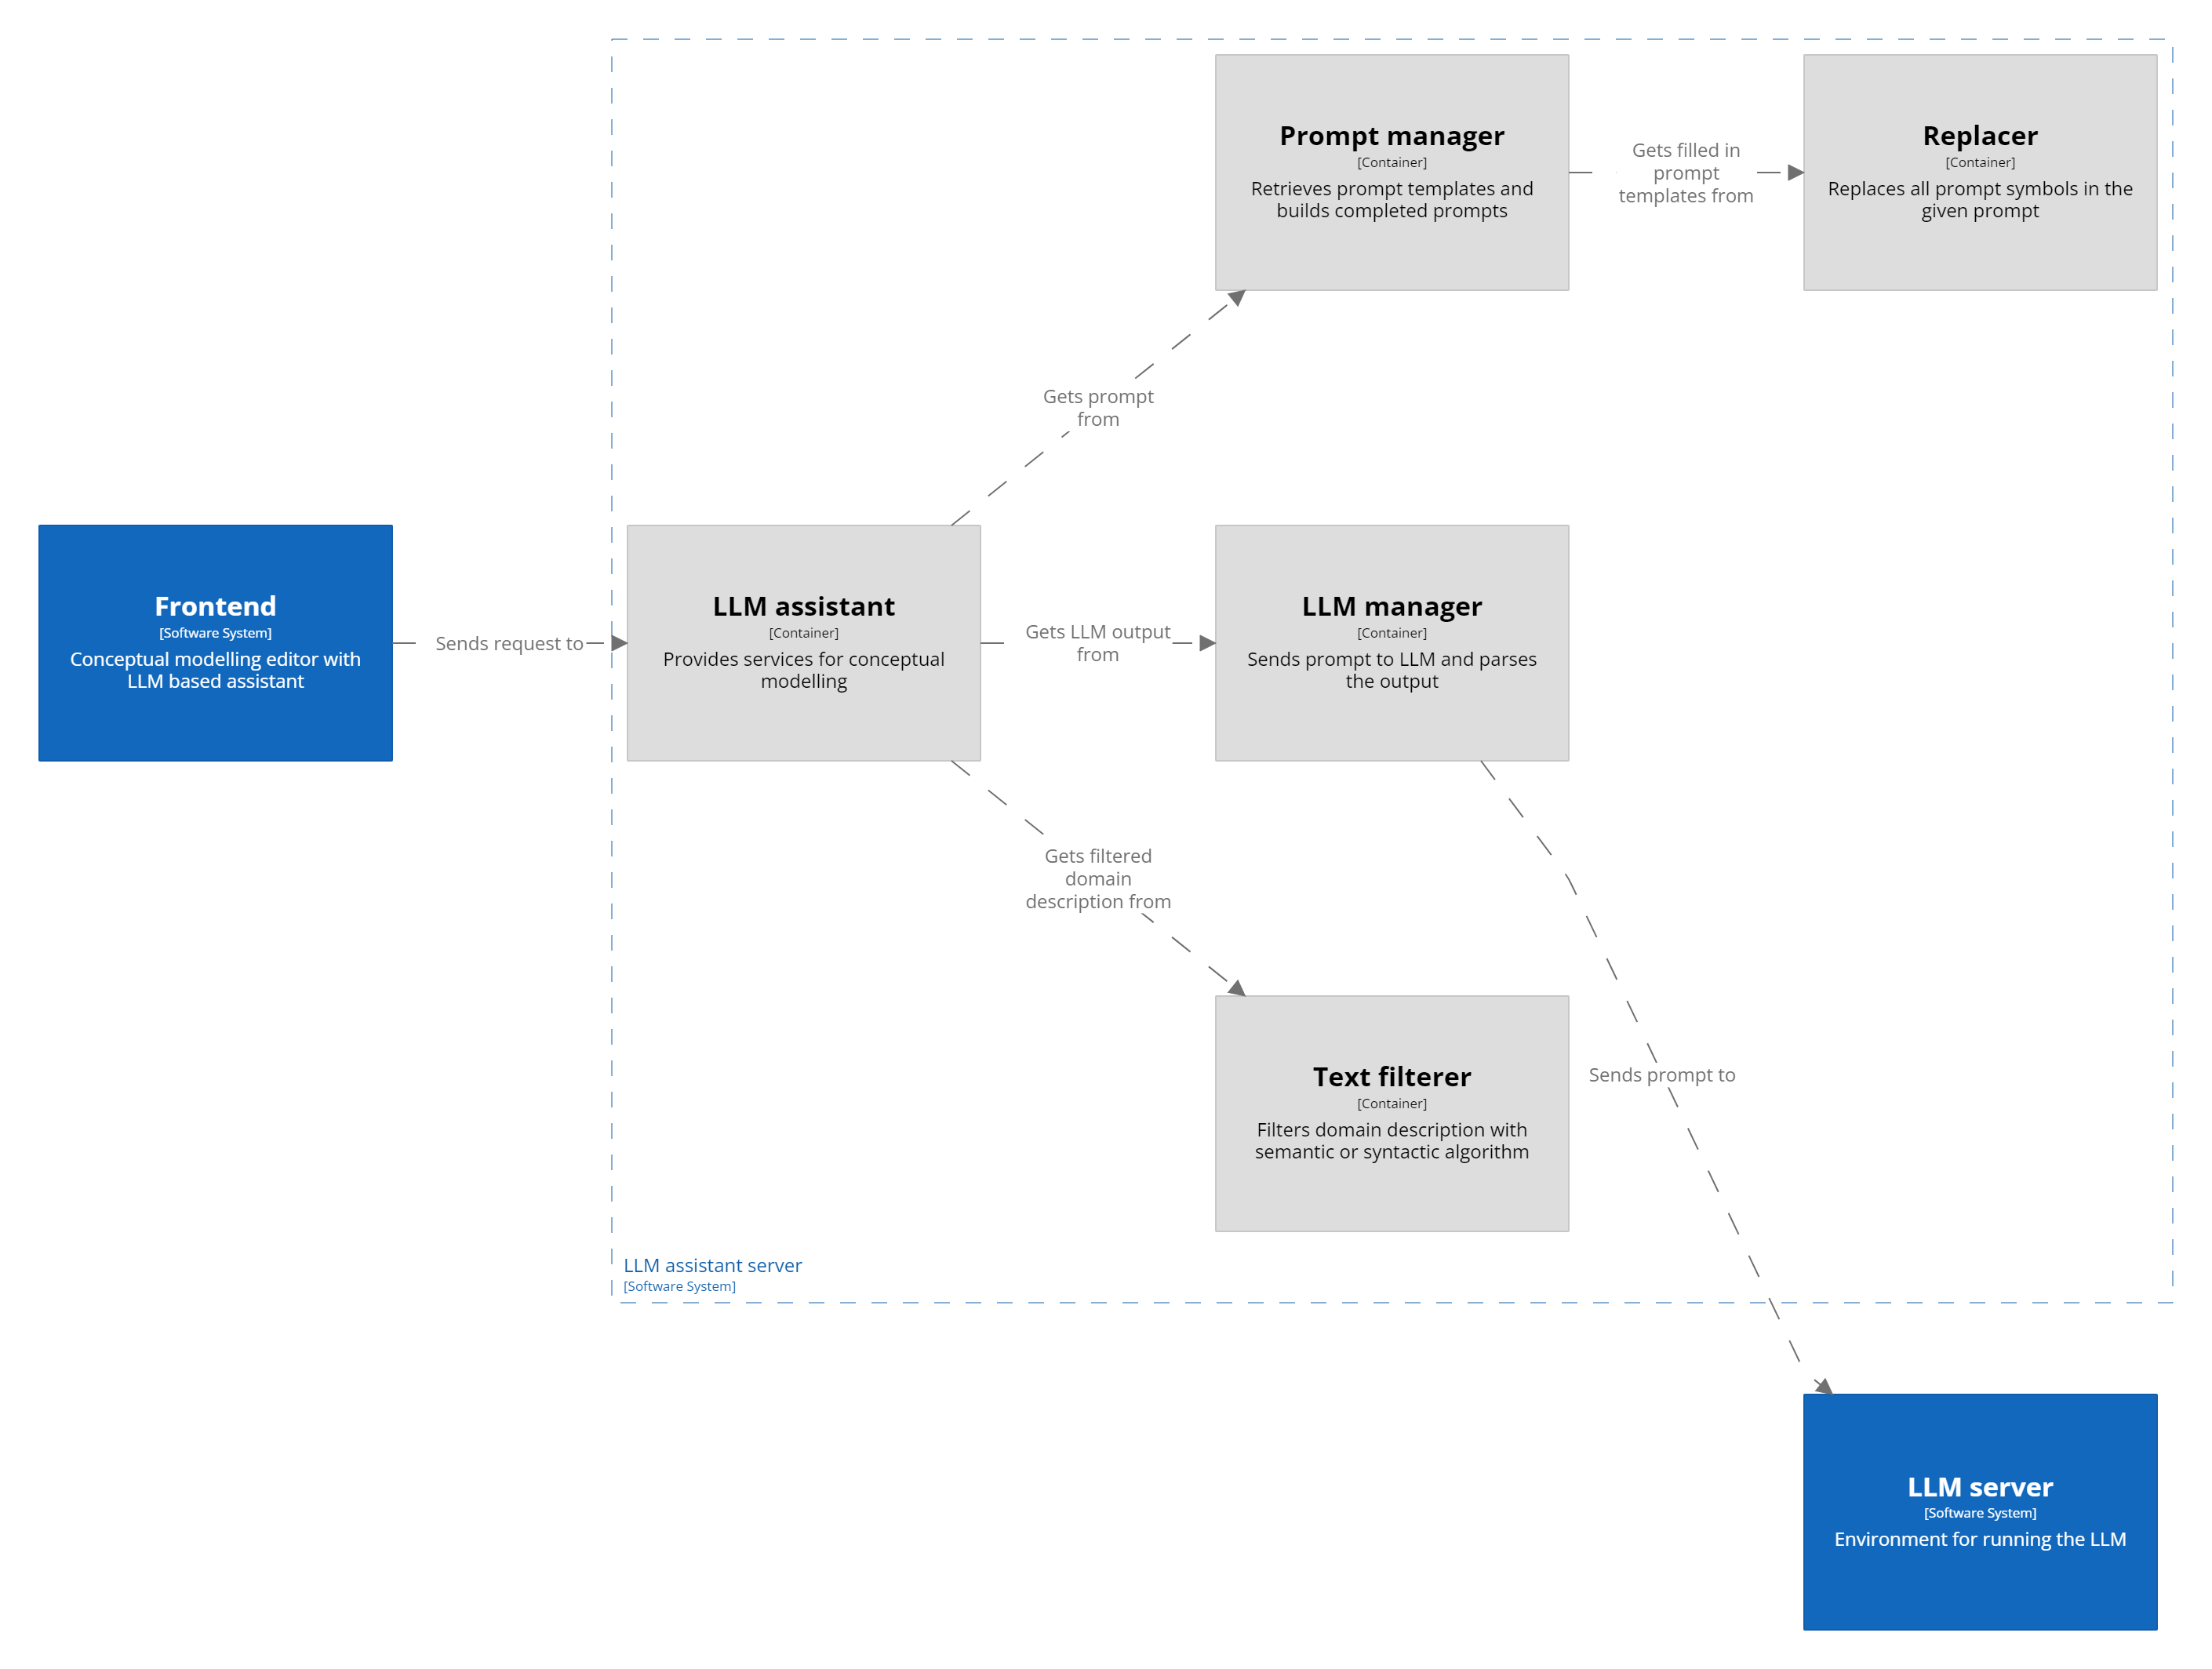
\includegraphics[scale=0.14]{../docs/images/architecture/llm-assistant-server-containers.png}
    \caption{\centering Architecture of the LLM assistant server}
    \label{fig:llm_assistant_server_containers}
\end{figure}

Now we describe the \emph{LLM assistant server} architecture shown on the picture \ref{fig:llm_assistant_server_containers} with the work-flow of the \emph{LLM assistant server}. When the user is creating his domain model on the frontend he can call our \emph{LLM assistant server} through the UI. When the \emph{LLM assistant server} is called a corresponding method is called on the instance of the \textit{LLMAssistant} class from the \textit{utils/llm\_assistant.py} script. Now the following tasks needs to be done:

\begin{enumerate}
\item get corresponding prompt template
\item fill in all prompt symbols (placeholders) in the prompt template
\item send this prompt to the LLM
\item parse the output from the LLM
\item show the output to the user
\end{enumerate}


\subsubsection{Prompt processing}

The \textit{LLMAssistant} uses an instance of the \textit{PromptManager} class from \textit{utils/prompt\_manager.py} to find the corresponding prompt template.
Then the class \textit{Replacer} from \textit{utils/replacer.py} replaces the prompt symbols defined inside \textit{definitions/prompt\_symbols.py} with the corresponding parameters sent from the frontend. Before the domain description is inserted it can be firstly filtered by either our semantic or syntactic RAG approach. First, the domain description is split into chunks by the class \textit{TextSplitter} from \textit{utils/text\_splitter.py}. The semantic algorithm uses an instance of the class \textit{SemanticTextFilterer} from \textit{text-filterer/semantic\_text\_filterer.py} it uses a language model from \textit{SentenceTransformers}\footnote{\url{https://sbert.net/}} library. The syntactic algorithm uses an instance of the class \textit{SyntacticTextFilterer} from \textit{text-filterer/syntactic\_text\_filterer.py}. It uses a language model from \textit{MorphoDiTa}\footnote{\url{https://pypi.org/project/ufal.morphodita/}} library. When all symbols in the prompt are filled in the prompt is ready to be sent to the LLM server.


\subsubsection{LLM output processing}

The \textit{LLMAssistant} uses the instance of the class \textit{LLMManager} from \textit{utils/llm\_manager.py} to send the prompt to the \emph{LLM server} and to parse the output. If the outputted object contains original text then an instance of the class \textit{OriginalTextFinder} from \textit{utils/original\_text\_finder.py} is used to find its original text indexes to highlight to the user this object in the domain description. The class \textit{OriginalTextFinder} is able to recover from some minor mistakes which is tested inside the script \textit{tests/find\_original\_text\_indexes.py}
also for consistency, we are automatically converting any generated name from any convention into the standard convention inside the script \textit{utils/convention\_convertor.py}. The correctness of this conversion is tested inside the \textit{tests/convention\_convertor.py} script. As soon as some object is generated by the LLM and approved by our scripts, it is sent back to the user on the frontend for a faster response time. If the user wants to highlight the parts of his domain description that he already covered with his domain model then the instance of the class \textit{OriginalTextMerger} is used to merge all original text indexes. Correctness of the merging is tested in \textit{tests/merge\_original\_text\_indexes.py}